\documentclass[11pt,a4paper]{article}

\usepackage[utf8]{inputenc}
\usepackage[T1]{fontenc}
\usepackage[english]{babel}
\usepackage[a4paper,margin=2.4cm]{geometry}

\usepackage{amsmath, amssymb, amsthm}
\usepackage{mathtools}
\usepackage{stmaryrd}
\usepackage{booktabs}
\usepackage{tabularx}
\usepackage{array}
\usepackage{caption}
\usepackage{subcaption}
\usepackage{float}
\usepackage{enumitem}
\usepackage{microtype}
\usepackage{xcolor}
\usepackage{listings}
\usepackage{fancyhdr}
\usepackage{titlesec}
\usepackage{graphicx}
\usepackage{tikz}
\usetikzlibrary{positioning, arrows.meta, fit, backgrounds, calc, shapes.geometric}
\usepackage[hidelinks]{hyperref}

%  ---  Palette shared with the companion reports  ---
\definecolor{ink}{RGB}{26,30,36}
\definecolor{slate}{RGB}{92,101,112}
\definecolor{mist}{RGB}{233,235,238}
\definecolor{rulegrey}{RGB}{188,194,201}
\definecolor{steel}{RGB}{47,72,102}
\definecolor{steellight}{RGB}{124,146,172}
\definecolor{signal}{RGB}{160,32,45}
\definecolor{pickc}{RGB}{51,115,204}
\definecolor{movec}{RGB}{230,128,38}
\definecolor{knows}{RGB}{26,140,70}

\hypersetup{
    colorlinks=true,
    linkcolor=steel,
    citecolor=steel,
    urlcolor=steel,
    pdftitle={A False Belief on a Warehouse Floor: The Sally-Anne Task for Two Robots},
    pdfauthor={Haniel Ulises},
}

\color{ink}

\setlength{\headheight}{22pt}
\pagestyle{fancy}
\fancyhf{}
\fancyhead[L]{\small\textcolor{slate}{\itshape A False Belief on a Warehouse Floor}}
\fancyhead[R]{\small\textcolor{slate}{\thepage}}
\renewcommand{\headrulewidth}{0.4pt}
\renewcommand{\headrule}{\hbox to\headwidth{\color{rulegrey}\leaders\hrule height \headrulewidth\hfill}}

\titleformat{\section}{\normalfont\large\bfseries\color{ink}}{\thesection}{0.7em}{}
\titleformat{\subsection}{\normalfont\normalsize\bfseries\color{ink}}{\thesubsection}{0.7em}{}
\titleformat{\paragraph}[runin]{\normalfont\bfseries\color{slate}}{}{0em}{}[.]

\captionsetup{font=small, labelfont={bf,color=slate}, textfont=footnotesize}

\theoremstyle{definition}
\newtheorem{definition}{Definition}
\newtheorem{proposition}{Proposition}
\newtheorem{lemma}{Lemma}
\newtheorem{corollary}{Corollary}
\newtheorem{fact}{Fact}
\newtheorem{remark}{Remark}

\lstdefinestyle{sys}{
    backgroundcolor=\color{mist},
    basicstyle=\ttfamily\scriptsize\color{ink},
    keywordstyle=\color{steel}\bfseries,
    commentstyle=\color{slate}\itshape,
    stringstyle=\color{slate},
    morecomment=[l]{;},
    morekeywords={:types,:predicates,:objects,:agents,:goal,:init,:event,:action,:action-type,:observability-conditions,:precondition,:effects,:events,:relations,:designated,:conditions,:observability-types},
    frame=single,
    rulecolor=\color{rulegrey},
    framesep=5pt,
    xleftmargin=6pt,
    xrightmargin=0pt,
    breaklines=true,
    showstringspaces=false,
    columns=fullflexible,
    captionpos=b,
}
\lstset{style=sys}

%  ---  Notation  ---
\newcommand{\Ag}{\mathcal{A}}
\newcommand{\Mod}{\mathcal{M}}
\newcommand{\Ev}{\mathcal{E}}
\newcommand{\prd}{\otimes}
\newcommand{\Bop}[1]{B_{#1}}
\newcommand{\Kop}[1]{K_{#1}}
\newcommand{\Cop}[1]{C_{#1}}
\newcommand{\code}[1]{\texttt{\small #1}}
\newcommand{\ag}[1]{\mathit{#1}}
\newcommand{\pk}{\ag{p}}
\newcommand{\mv}{\ag{m}}
\newcommand{\crate}{\mathit{crate}}
\newcommand{\pre}{\mathit{pre}}
\newcommand{\post}{\mathit{post}}
\newcommand{\sem}[1]{\llbracket #1 \rrbracket}

\begin{document}

\begin{titlepage}
\centering
\vspace*{2.4cm}
{\color{rulegrey}\rule{\textwidth}{0.8pt}}\\[0.9cm]
{\LARGE\bfseries A False Belief on a Warehouse Floor\par}
\vspace{0.5cm}
{\large\color{slate} A Relocation One Robot Does Not See, an Observation\\
Its Beliefs Rule Out, and a Report That Repairs Them\par}
\vspace{0.7cm}
{\color{rulegrey}\rule{\textwidth}{0.8pt}}\\[1.4cm]

{\large Haniel Ulises\par}
\vspace{0.3cm}
{\color{slate} Epistemic Robotics}\\
\vspace{0.15cm}
{\color{slate}\today}

\vfill
{\color{slate}\small
A crate is moved from one bay to another while the robot that stored it is
charging out of sight of both, and the robot that moved it has to reason about
where the other will look. The setting follows the false-belief tasks of
developmental psychology, the Sally-Anne test in particular, as formalised in
dynamic epistemic logic by Bolander. We state it as a planning domain over
$\mathrm{KD45}$ models and prove four things about it. A relocation the picker
does not observe leaves it believing the crate is where it was, and the mover
believing that it believes so. An observation or a truthful announcement that
contradicts a belief leaves the believer with no accessible world, so that it
believes every formula, and a planner that requires consistent beliefs refuses
such an update. A report the picker takes as news of the move repairs its belief
consistently and yields common belief of the new location. A picker that allows
the move without seeing it is uncertain and not wrong, and finds the crate by
looking. The planner reproduces each: with a radio it plans the report, without
one it finds no policy, and with a doubting picker it plans a look before the
fetch. All three floors were executed in Gazebo through ePlanSys. Without the
report the picker drove to the bay it believed the crate was in, the bay the
mover's model predicted, and found it empty.}
\vspace{1.2cm}
\end{titlepage}

\tableofcontents
\newpage

%  ======================================================================
\section{Scope}
\label{sec:scope}

The false-belief task asks whether a subject can attribute to someone else a
belief the subject knows to be false~\cite{wimmer1983}. In the Sally-Anne
version~\cite{baroncohen1985}, Sally puts a marble in a basket and leaves; Anne
moves it to a box; the subject is asked where Sally will look for it. The right
answer is the basket, where Sally believes it is, and not the box, where the
subject knows it is. Bolander~\cite{bolander2018} formalises the task in
dynamic epistemic logic: the move is an action Sally does not observe, the
model after it has Sally believing something false, and the question is a
formula of the form $\Bop{\mathit{Anne}}\Bop{\mathit{Sally}}\varphi$ evaluated on
that model.

This report puts the task on the pass-through floor of the companion reports,
with two robots. The \emph{picker} stores a crate in bay $t_1$ and goes to
charge at a dock from which neither bay is in sight; the \emph{mover} carries
the crate to $t_3$; the picker is then to fetch it. What the report establishes:

\begin{itemize}[leftmargin=1.4em, itemsep=2pt]
  \item The relocation planted a false belief, and the mover's model
    attributed it: after the move the crate is in $t_3$, the picker believes it
    in $t_1$, and the mover believes the picker believes so
    (Proposition~\ref{prop:false}). The planner and the epistemic state compute
    this model by product update; it is not written down.
  \item An observation the picker's beliefs rule out, such as finding $t_1$
    empty, or a truthful announcement of where the crate is, leaves the picker
    with no accessible world (Proposition~\ref{prop:collapse}). A planner
    that admits such a state finds a policy that relies on it; one that
    requires consistent beliefs finds none on the floor without a radio, and
    the planner returns none.
  \item A report the picker takes as news of the move repairs its belief and
    yields common belief of the new location (Proposition~\ref{prop:report});
    with a radio the planner places it before the fetch.
  \item A picker that allows the move without seeing it has no false belief to
    repair, and finds the crate by looking (Proposition~\ref{prop:doubt}).
  \item All three floors were executed in Gazebo through ePlanSys, and on the
    floor without a radio the picker drove to $t_1$ and found it empty
    (Section~\ref{sec:runs}).
\end{itemize}

\noindent
Not established: belief revision. When an observation contradicts a belief,
the logic used here has no answer short of the empty relation;
plausibility models~\cite{baltag2008} give one, and are outside what the
planner implements. The crate is moved by the simulator once a robot is in
position to carry it: the robots have no gripper.

%  ======================================================================
\section{Preliminaries}
\label{sec:prelim}

\begin{definition}[Epistemic model]
Let $\Ag$ be a finite set of agents and $P$ a finite set of atoms. A model is
$\Mod = (W, R, V, W_d)$ with $W$ a finite set of worlds,
$R : \Ag \to 2^{W\times W}$, $V : W \to 2^P$ and $\emptyset \neq W_d \subseteq W$
the designated worlds. It is $\mathrm{S5}$ when every $R_a$ is an equivalence,
and $\mathrm{KD45}$ when every $R_a$ is serial, transitive and Euclidean. A
formula holds at $\Mod$ when it holds at every designated world.
\end{definition}

\begin{definition}[Belief]
$\Mod, w \models \Bop{a}\varphi$ iff $\Mod, v \models \varphi$ for every $v$ with
$w R_a v$. For a group $G$, $\Cop{G}\varphi$ quantifies over the worlds reachable
from $w$ by one or more steps of $\bigcup_{a\in G} R_a$. Over $\mathrm{S5}$ models
$\Bop{a}$ is knowledge and is written $\Kop{a}$; over $\mathrm{KD45}$ models it
is belief, which can be false. The tools write both as \code{[a]}.
\end{definition}

\begin{definition}[Consistent belief]
\label{def:consistent}
Agent $a$ has a \emph{consistent belief} at $w$ if $R_a(w) \neq \emptyset$. If
$R_a(w) = \emptyset$, then $\Mod, w \models \Bop{a}\varphi$ for every $\varphi$,
$\bot$ included: $a$ believes everything. A model in which every world reachable
from $W_d$ has a successor for every agent is \emph{consistent}.
\end{definition}

\begin{definition}[Event model and product update~\cite{baltag1998}]
An event model is $\Ev = (E, T, Q, \pre, \post, E_d)$ with events $E$,
observability types $T$, $Q : T \to 2^{E\times E}$, preconditions, postconditions
and designated events $E_d$. Each agent $a$ is given a type $\tau_a$ for the
whole model, the type whose condition holds at the designated worlds, as plank
and Aletheia evaluate it. Then $\Mod \prd \Ev = (W', R', V', W'_d)$ with
$W' = \{(w,e) : \Mod, w \models \pre(e)\}$,
$(w,e)\, R'_a\, (v,f)$ iff $w R_a v$ and $(e,f) \in Q(\tau_a)$, $V'$ given by
the postconditions, and $W'_d = \{(w,e) \in W' : w \in W_d, e \in E_d\}$.
\end{definition}

\begin{lemma}
\label{lem:kd45}
If $R_a$ and $Q(\tau_a)$ are transitive, so is $R'_a$; if both are Euclidean, so
is $R'_a$; if both are equivalences, so is $R'_a$. Seriality is not preserved:
$(w,e)$ has no $a$-successor whenever no $v \in R_a(w)$ satisfies the
precondition of any $f$ with $(e,f) \in Q(\tau_a)$.
\end{lemma}

\begin{proof}
If $(w,e) R'_a (v,f) R'_a (u,g)$ then $w R_a u$ and $(e,g) \in Q(\tau_a)$ by
transitivity of each, and $(u,g) \in W'$, so $(w,e) R'_a (u,g)$. If $(w,e)$
reaches both $(v,f)$ and $(u,g)$ then $v R_a u$ and $(f,g) \in Q(\tau_a)$ by
Euclideanness of each, so $(v,f) R'_a (u,g)$. Reflexivity and symmetry carry over
in the same way on the worlds that survive. The last claim is the definition of
$R'_a$ with an empty set of candidates~\cite{vanditmarsch2007}.
\end{proof}

\noindent
Aletheia offers three treatments of a product that loses seriality: keep it, as
plank does (\code{Ignore}, the default); delete the worlds that lost it
(\code{Repair}); or refuse the update (\code{Require}, enabled by
\code{--consistent-beliefs}). The planner of this report runs with
\code{Require}, and ePlanSys's planner plugin sets it by default. The epistemic
state that tracks the run applies updates with \code{Ignore}
(Section~\ref{sec:defects}).

%  ======================================================================
\section{The domain}
\label{sec:domain}

Agents $\pk$ (picker) and $\mv$ (mover); bays $t_1$ and $t_3$; atoms
$\crate(b)$ for each bay, $\mathit{at\text{-}dock}(\pk)$, $\mathit{fetched}$,
the static facts $\mathit{radio}$ and $\mathit{doubts}$, and two phase atoms.
Initially every atom is common knowledge, the crate is in $t_1$, and the model
has one world. The goal is $\mathit{fetched}$.

\paragraph{The shift} Its first two actions are not chosen by the planner. The
picker goes to its dock, a public ontic action; then the mover carries the crate
from $t_1$ to $t_3$. Two phase atoms hold that order, and every later action
requires both cleared.

\begin{definition}[Relocation]
\label{def:relocation}
$\mathit{Rel}(\mv, a, b)$ has events $\delta$ (the move) and $\sigma$ (the
mover's slot passing with nothing moved), with
$\pre(\delta) = \crate(a) \wedge \neg\crate(b) \wedge \mathit{due}$,
$\post(\delta) : \crate(b), \neg\crate(a), \neg\mathit{due}$, and
$\pre(\sigma) = \mathit{due}$, $\post(\sigma) : \neg\mathit{due}$. Designated
$\{\delta\}$. Three types:
$Q(\mathrm{Fully}) = \{(\delta,\delta),(\sigma,\sigma)\}$,
$Q(\mathrm{Doubting}) = \{\delta,\sigma\}^2$,
$Q(\mathrm{Oblivious}) = \{(\delta,\sigma),(\sigma,\sigma)\}$.
The mover is Fully; the picker is Doubting if $\mathit{doubts}$ holds and
Oblivious otherwise.
\end{definition}

\noindent
The event $\sigma$ carries the phase change because the picker knows the
schedule: it knows the mover's slot has passed, and does not know the mover
used it. A first version left $\sigma$ trivial, and the phase atom then stayed
set in every world the picker considered possible
(Section~\ref{sec:defects}).

\begin{definition}[Report]
\label{def:report}
$\mathit{Rep}(\mv, \pk, a, b)$ has events $\rho$ (the report) and $\mu$ (the
move, as the picker takes it), with
$\pre(\rho) = \mathit{radio} \wedge \crate(b) \wedge \Bop{\mv}\crate(b) \wedge
\Bop{\mv}\Bop{\pk}\crate(a)$, trivial postconditions, and
$\pre(\mu) = \crate(a)$, $\post(\mu) : \crate(b), \neg\crate(a)$. Designated
$\{\rho\}$. Types $Q(\mathrm{Fully}) = \{(\rho,\rho),(\mu,\mu)\}$ for the mover
and $Q(\mathrm{Recipient}) = \{(\rho,\mu),(\mu,\mu)\}$ for the picker.
\end{definition}

\noindent
The precondition $\Bop{\mv}\Bop{\pk}\crate(a)$ is the false-belief test as a
precondition: the mover reports only what it believes the picker believes
otherwise.

\begin{figure}[H]
\centering
\begin{subfigure}[b]{0.47\textwidth}
\centering
\begin{tikzpicture}[
  ev/.style={draw, rounded corners=3pt, minimum width=1.6cm, minimum height=0.75cm, fill=mist, font=\small},
  des/.style={ev, draw=signal, line width=1.3pt},
  lab/.style={font=\scriptsize, text=slate}]
\node[des] (d) at (0,0) {$\delta$};
\node[ev] (s) at (3.4,0) {$\sigma$};
\draw[-{Stealth}, pickc, line width=1.4pt] (d) -- node[above, font=\small] {$\pk$} (s);
\draw[-{Stealth}, pickc, line width=1.1pt] (s.north east) .. controls +(0.6,0.8) and +(-0.6,0.8) .. (s.north west);
\node[lab, below=0.15cm of d] {$\crate(t_1) \mapsto \crate(t_3)$};
\node[lab, below=0.15cm of s] {nothing moved};
\end{tikzpicture}
\caption{Oblivious: the picker takes the move for nothing having moved.}
\end{subfigure}\hfill
\begin{subfigure}[b]{0.47\textwidth}
\centering
\begin{tikzpicture}[
  ev/.style={draw, rounded corners=3pt, minimum width=1.6cm, minimum height=0.75cm, fill=mist, font=\small},
  des/.style={ev, draw=signal, line width=1.3pt},
  lab/.style={font=\scriptsize, text=slate}]
\node[des] (d) at (0,0) {$\delta$};
\node[ev] (s) at (3.4,0) {$\sigma$};
\draw[pickc, line width=1.4pt] (d) -- node[above, font=\small] {$\pk$} (s);
\node[lab, below=0.15cm of d] {$\crate(t_1) \mapsto \crate(t_3)$};
\node[lab, below=0.15cm of s] {nothing moved};
\end{tikzpicture}
\caption{Doubting: the picker relates the two, and is left uncertain.}
\end{subfigure}
\caption{The relocation $\mathit{Rel}(\mv, t_1, t_3)$ under the picker's two
types. Reflexive edges of the mover are omitted; the mover is Fully.}
\label{fig:relocation}
\end{figure}

\noindent
The remaining actions: $\mathit{look}(\pk, b)$ is semi-private sensing with
events $\crate(b)$ and $\neg\crate(b)$, the picker Fully and the mover
Partially; $\mathit{fetch}(\pk, b)$ is public and ontic with precondition
$\crate(b) \wedge \Bop{\pk}\crate(b)$: the picker drives to the bay only if it
believes the crate is there. The three floors are three instances that differ in
two lines:

\begin{table}[H]
\centering\small
\caption{The three instances.}
\label{tab:floors}
\begin{tabular}{@{}l l l@{}}
\toprule
instance & $\mathit{radio}$ & $\mathit{doubts}$ \\
\midrule
\code{told} & true & false \\
\code{untold} & false & false \\
\code{doubt} & false & true \\
\bottomrule
\end{tabular}
\end{table}

\begin{lstlisting}[caption={The two action types, in \code{epddl/beliefs.epddl}.}, label={lst:beliefs}]
(:action-type relocation
  :events     (?do ?skip)
  :observability-types (Fully Doubting Oblivious)
  :relations  (Fully     (:forall (?e - event) (?e ?e))
               Doubting  (:forall (?e ?f - event) (?e ?f))
               Oblivious (:forall (?e - event) (?e ?skip)) )
  :designated (?do)
  :conditions (?do (:non-trivial-postconditions)))

(:action-type report
  :events     (?told ?revise)
  :observability-types (Fully Recipient)
  :relations  (Fully     (:forall (?e - event) (?e ?e))
               Recipient (:and (?told ?revise) (?revise ?revise)) )
  :designated (?told)
  :conditions (?told (:trivial-postconditions)
               ?revise (:non-trivial-postconditions)))
\end{lstlisting}

%  ======================================================================
\section{The false belief}
\label{sec:false}

Let $\Mod_0$ be the model after the picker has gone to its dock: one world $w$,
$\crate(t_1)$ true, both relations $\{(w,w)\}$.

\begin{proposition}[A false belief, and its attribution]
\label{prop:false}
Let $\Mod_1 = \Mod_0 \prd \mathit{Rel}(\mv, t_1, t_3)$ with the picker Oblivious.
Then $\Mod_1$ is $\mathrm{KD45}$ and not $\mathrm{S5}$, and at its designated world
\[
  \crate(t_3) \wedge \Bop{\pk}\crate(t_1) \wedge \Bop{\mv}\crate(t_3)
  \wedge \Bop{\mv}\Bop{\pk}\crate(t_1) \wedge \Bop{\pk}\Bop{\mv}\crate(t_1).
\]
\end{proposition}

\begin{proof}
Both events apply at $w$, so $W_1 = \{(w,\delta), (w,\sigma)\}$ with
$\crate(t_3)$ at the first and $\crate(t_1)$ at the second, and the first
designated. The mover is Fully: $R_\mv = \{((w,\delta),(w,\delta)),
((w,\sigma),(w,\sigma))\}$. The picker is Oblivious:
$R_\pk = \{((w,\delta),(w,\sigma)), ((w,\sigma),(w,\sigma))\}$, serial,
transitive and Euclidean, and not reflexive at $(w,\delta)$. At $(w,\delta)$:
the picker's only world has $\crate(t_1)$; the mover's only world is
$(w,\delta)$ itself, with $\crate(t_3)$, from which the picker's only world has
$\crate(t_1)$; and the picker's world $(w,\sigma)$ is the mover's only world
from itself, with $\crate(t_1)$.
\end{proof}

\noindent
The last conjunct is the picker believing the mover shares its belief: in the
world the picker believes, nothing happened to anyone. The fourth is the answer
to the Sally-Anne question. Where will the picker look? Where the mover believes
it believes the crate is: $t_1$.

%  ======================================================================
\section{An observation the belief rules out}
\label{sec:collapse}

\begin{proposition}[No consistent update]
\label{prop:collapse}
Let $\Mod, w \models \Bop{a}\neg\psi$, and let $\Ev$ be an event model in which
$a$ is Fully and $e$ an event with $\Mod, w \models \pre(e)$ and
$\pre(e) \models \psi$. Then $R'_a((w,e)) = \emptyset$ in $\Mod \prd \Ev$.
\end{proposition}

\begin{proof}
$R'_a((w,e)) = \{(v,f) : w R_a v,\ (e,f) \in Q(\mathrm{Fully}),\ \Mod, v \models
\pre(f)\}$. Fully relates $e$ only to $e$, so $f = e$; and every $v \in R_a(w)$
satisfies $\neg\psi$, hence not $\pre(e)$.
\end{proof}

\begin{corollary}[The untold floor]
\label{cor:untold}
On \code{untold}, after the shift's two actions, no action leads to a
consistent state in which $\mathit{fetched}$ can be reached. Hence there is no
policy when consistent beliefs are required.
\end{corollary}

\begin{proof}
In $\Mod_1$ the picker believes $\crate(t_1) \wedge \neg\crate(t_3)$. The report
is inapplicable without $\mathit{radio}$. $\mathit{fetch}(\pk, t_1)$ needs
$\crate(t_1)$, false at the designated world, and $\mathit{fetch}(\pk, t_3)$
needs $\Bop{\pk}\crate(t_3)$, false. $\mathit{look}(\pk, t_1)$ has, at the
designated world, only the event of $\neg\crate(t_1)$, and
$\mathit{look}(\pk, t_3)$ only that of $\crate(t_3)$; the picker is Fully and
believes the negation of each, so by Proposition~\ref{prop:collapse} either
look leaves it with no world, and is refused.
\end{proof}

\noindent
A truthful public announcement of $\crate(t_3)$ falls under the same
proposition: every agent is Fully and the picker believes $\neg\crate(t_3)$.
That is why the report is not an announcement.

\begin{remark}
\label{rem:vacuous}
Under \code{Ignore} the look is applied and the picker believes everything,
$\Bop{\pk}\crate(t_3)$ included, which makes $\mathit{fetch}(\pk, t_3)$
applicable. Aletheia run without \code{--consistent-beliefs} returns exactly
that policy on \code{untold}: look into $t_1$, then fetch from $t_3$, on a
belief that holds vacuously. Run with it, it returns none.
\end{remark}

%  ======================================================================
\section{The report}
\label{sec:report}

\begin{proposition}[A report that repairs the belief]
\label{prop:report}
$\mathit{Rep}(\mv, \pk, t_1, t_3)$ is applicable in $\Mod_1$, and
$\Mod_2 = \Mod_1 \prd \mathit{Rep}(\mv, \pk, t_1, t_3)$ is consistent and satisfies
$\Bop{\pk}\crate(t_3) \wedge \Cop{\{\pk,\mv\}}\crate(t_3)$.
\end{proposition}

\begin{proof}
At $(w,\delta)$, $\crate(t_3)$ and $\Bop{\mv}\crate(t_3)$ hold, and
$\Bop{\mv}\Bop{\pk}\crate(t_1)$ holds by Proposition~\ref{prop:false}: $\rho$
applies there, and only there, since $\crate(t_3)$ fails at $(w,\sigma)$; $\mu$
applies only at $(w,\sigma)$. So $W_2 = \{x, y\}$ with $x = ((w,\delta),\rho)$
designated and $y = ((w,\sigma),\mu)$, and $\crate(t_3)$ holds at both, at $y$ by
$\post(\mu)$. The picker relates $\rho$ to $\mu$ and $\mu$ to $\mu$, and
$(w,\delta) R_\pk (w,\sigma) R_\pk (w,\sigma)$, so $R_\pk = \{(x,y),(y,y)\}$; the
mover is Fully and $R_\mv = \{(x,x),(y,y)\}$. Every world has a successor for
each agent, both worlds satisfy $\crate(t_3)$, and they are all the worlds
reachable from $x$.
\end{proof}

\noindent
The picker takes the report as the move it did not see, applied to the world
it believes, and its belief is then true. Its relation is still not reflexive:
it believes the crate moved just now, and it moved earlier. Nothing the picker
believes about the crate is false.

%  ======================================================================
\section{Doubt}
\label{sec:doubt}

\begin{proposition}[Uncertain, not wrong]
\label{prop:doubt}
Let $\Mod'_1 = \Mod_0 \prd \mathit{Rel}(\mv, t_1, t_3)$ with the picker Doubting.
Then $\Mod'_1$ is $\mathrm{S5}$, the picker believes the crate in neither bay,
and after $\mathit{look}(\pk, t_1)$ with the outcome $\neg\crate(t_1)$ the model
is consistent and satisfies $\Kop{\pk}\crate(t_3)$.
\end{proposition}

\begin{proof}
The worlds are those of Proposition~\ref{prop:false}; the picker's relation is
now $\{(w,\delta),(w,\sigma)\}^2$, an equivalence, and the mover's the
identity. The two worlds disagree on the crate, so the picker believes neither
location. The look's negative event applies at $(w,\delta)$ and its positive
event at $(w,\sigma)$; the picker is Fully, so the two products are unrelated,
and from the designated $((w,\delta),\neg)$ the picker sees only itself, where
$\crate(t_3)$ holds.
\end{proof}

%  ======================================================================
\section{Planning results}
\label{sec:planning}

The task is epistemic planning in the sense of Bolander and
Andersen~\cite{bolander2011}. plank grounds each instance into 13 atoms and 18
ground actions. Aletheia, with consistent beliefs required, returns:

\begin{table}[H]
\centering\small
\caption{Planner results, with \code{--consistent-beliefs}.}
\label{tab:planning}
\begin{tabularx}{\textwidth}{@{}l X r@{}}
\toprule
instance & policy & depth \\
\midrule
\code{told} & go-dock, relocate, report($\mv$, $\pk$, $t_1$, $t_3$), fetch($\pk$, $t_3$) & 4 \\
\code{untold} & none: space exhausted & 3 \\
\code{doubt} & go-dock, relocate, look($\pk$, $t_1$), fetch($\pk$, $t_3$) & 4 \\
\bottomrule
\end{tabularx}
\end{table}

\noindent
Without \code{--consistent-beliefs} \code{untold} has the policy of
Remark~\ref{rem:vacuous}. \code{tools/validate.sh} checks six statements
without a simulator: the false belief and its attribution after the shift's two
actions; the told policy and its consistency at every node; no policy on
\code{untold}; the collapse after the look; the vacuous policy without
consistent beliefs, and that the trace finds the collapse in it; and the doubt
policy, with the picker uncertain and its relation reflexive after the move.

%  ======================================================================
\section{Grounding on the floor}
\label{sec:floor}

The floor is the pass-through floor: a racking block across the hall with
three tunnel bays, $t_1$, $t_2$ and $t_3$, the storage floor below it and the
dispatch floor above. The crate starts in $t_1$. The picker works the storage
floor and reaches a bay from its south mouth; the mover works the dispatch floor
and reaches it from the north. The dock is against the west wall between two
rows of racking.

The domain makes three claims about the floor, and \code{make\_floorplan.py}
checks each by casting rays over the occupied cells before writing the plan:
from the dock neither bay is in sight; from either mouth a robot sees along the
bay to the crate's place and through to the far floor; and every place a robot
is sent is reachable over the inflated plan. The performers check the first
again at run time: \code{go\_dock} logs which bays are in line of sight once
the picker is docked, and \code{relocate} logs, when it sets the crate down,
which bays are in sight of where the picker stands, and refuses if one is.

Looking into a bay is the picker's laser, read straight along the bay's axis
from its mouth: a crate reads at about three metres, an empty bay through to
the dispatch floor. \code{fetch} reads the same before it drives in, and
refuses if the bay is empty, whatever the model says. The crate rides on the
robot that carries it, moved through \code{gazebo\_ros\_state}.

%  ======================================================================
\section{Runs}
\label{sec:runs}

The three floors were recorded on a $3840 \times 1080$ virtual display with
RViz on the left and Gazebo on the right, and composed into one film whose
captions are the lines the runs wrote. In the tables the model column gives
worlds and designated worlds after the update, and the picker's belief.

\subsection{Untold}

\begin{table}[H]
\centering\small
\caption{The untold floor, as the run reported it.}
\label{tab:untold-run}
\begin{tabularx}{\textwidth}{@{}l X r@{}}
\toprule
action & reported & model \\
\midrule
plan & no policy for $\mathit{fetched}$ after 0.1\,s; space exhausted at depth 3 & 1 / 1 \\
$\mathit{go\text{-}dock}(\pk)$ & at its dock after 33\,s; bays in line of sight: $t_1$ no, $t_3$ no & 1 / 1 \\
$\mathit{relocate}(\mv, t_1, t_3)$ & takes the crate from $t_1$ after 56\,s, sets it down in $t_3$ after 124\,s; in sight of the picker: neither bay & 2 / 1, $\Bop{\pk}\,t_1$ \\
$\mathit{fetch}(\pk, t_1)$ & belief requirement held, dispatched; at the mouth of $t_1$ after 34\,s the laser read 11.2\,m: empty; refused by the performer & refused \\
\bottomrule
\end{tabularx}
\end{table}

\noindent
The mission then asked the epistemic state four questions and reported the
floor as the expected outcome on the answers: the crate is in $t_3$; the picker
believes it in $t_1$; the mover believes the picker believes so; the picker
believes the mover believes it in $t_1$. These are the four conjuncts of
Proposition~\ref{prop:false}, evaluated on the model the executor kept.

\subsection{Told}

\begin{table}[H]
\centering\small
\caption{The told floor, as the run reported it.}
\label{tab:told-run}
\begin{tabularx}{\textwidth}{@{}l X r@{}}
\toprule
action & reported & model \\
\midrule
plan & 4 policy items, 1 leaf, 0.1\,s & 1 / 1 \\
$\mathit{go\text{-}dock}(\pk)$ & at its dock after 35\,s; bays in line of sight: $t_1$ no, $t_3$ no & 1 / 1 \\
$\mathit{relocate}(\mv, t_1, t_3)$ & takes the crate from $t_1$ after 57\,s, sets it down in $t_3$ after 128\,s; in sight of the picker: neither bay & 2 / 1, $\Bop{\pk}\,t_1$ \\
$\mathit{report}(\mv, \pk, t_1, t_3)$ & ``the crate was moved from $t_1$ to $t_3$'', delivered and acknowledged & 2 / 1, $\Bop{\pk}\,t_3$ \\
$\mathit{fetch}(\pk, t_3)$ & at the mouth of $t_3$ after 71\,s the laser read 3.1\,m: the crate; set down at the drop 131\,s after fetch began & fetched \\
\bottomrule
\end{tabularx}
\end{table}

\subsection{Doubt}

\begin{table}[H]
\centering\small
\caption{The doubt floor, as the run reported it.}
\label{tab:doubt-run}
\begin{tabularx}{\textwidth}{@{}l X r@{}}
\toprule
action & reported & model \\
\midrule
plan & 4 policy items, 1 leaf, 0.1\,s & 1 / 1 \\
$\mathit{go\text{-}dock}(\pk)$ & at its dock after 36\,s; bays in line of sight: $t_1$ no, $t_3$ no & 1 / 1 \\
$\mathit{relocate}(\mv, t_1, t_3)$ & takes the crate from $t_1$ after 58\,s, sets it down in $t_3$ after 129\,s & 2 / 1, neither \\
$\mathit{look}(\pk, t_1)$ & at the mouth of $t_1$ after 33\,s the laser read 11.2\,m: empty, $e$-empty & 2 / 1, $\Kop{\pk}\,t_3$ \\
$\mathit{fetch}(\pk, t_3)$ & at the mouth of $t_3$ after 46\,s the laser read 3.1\,m: the crate; set down at the drop 108\,s after fetch began & fetched \\
\bottomrule
\end{tabularx}
\end{table}

\noindent
Every node of the three runs exited cleanly when the launch shut down.

\begin{figure}[H]
\centering
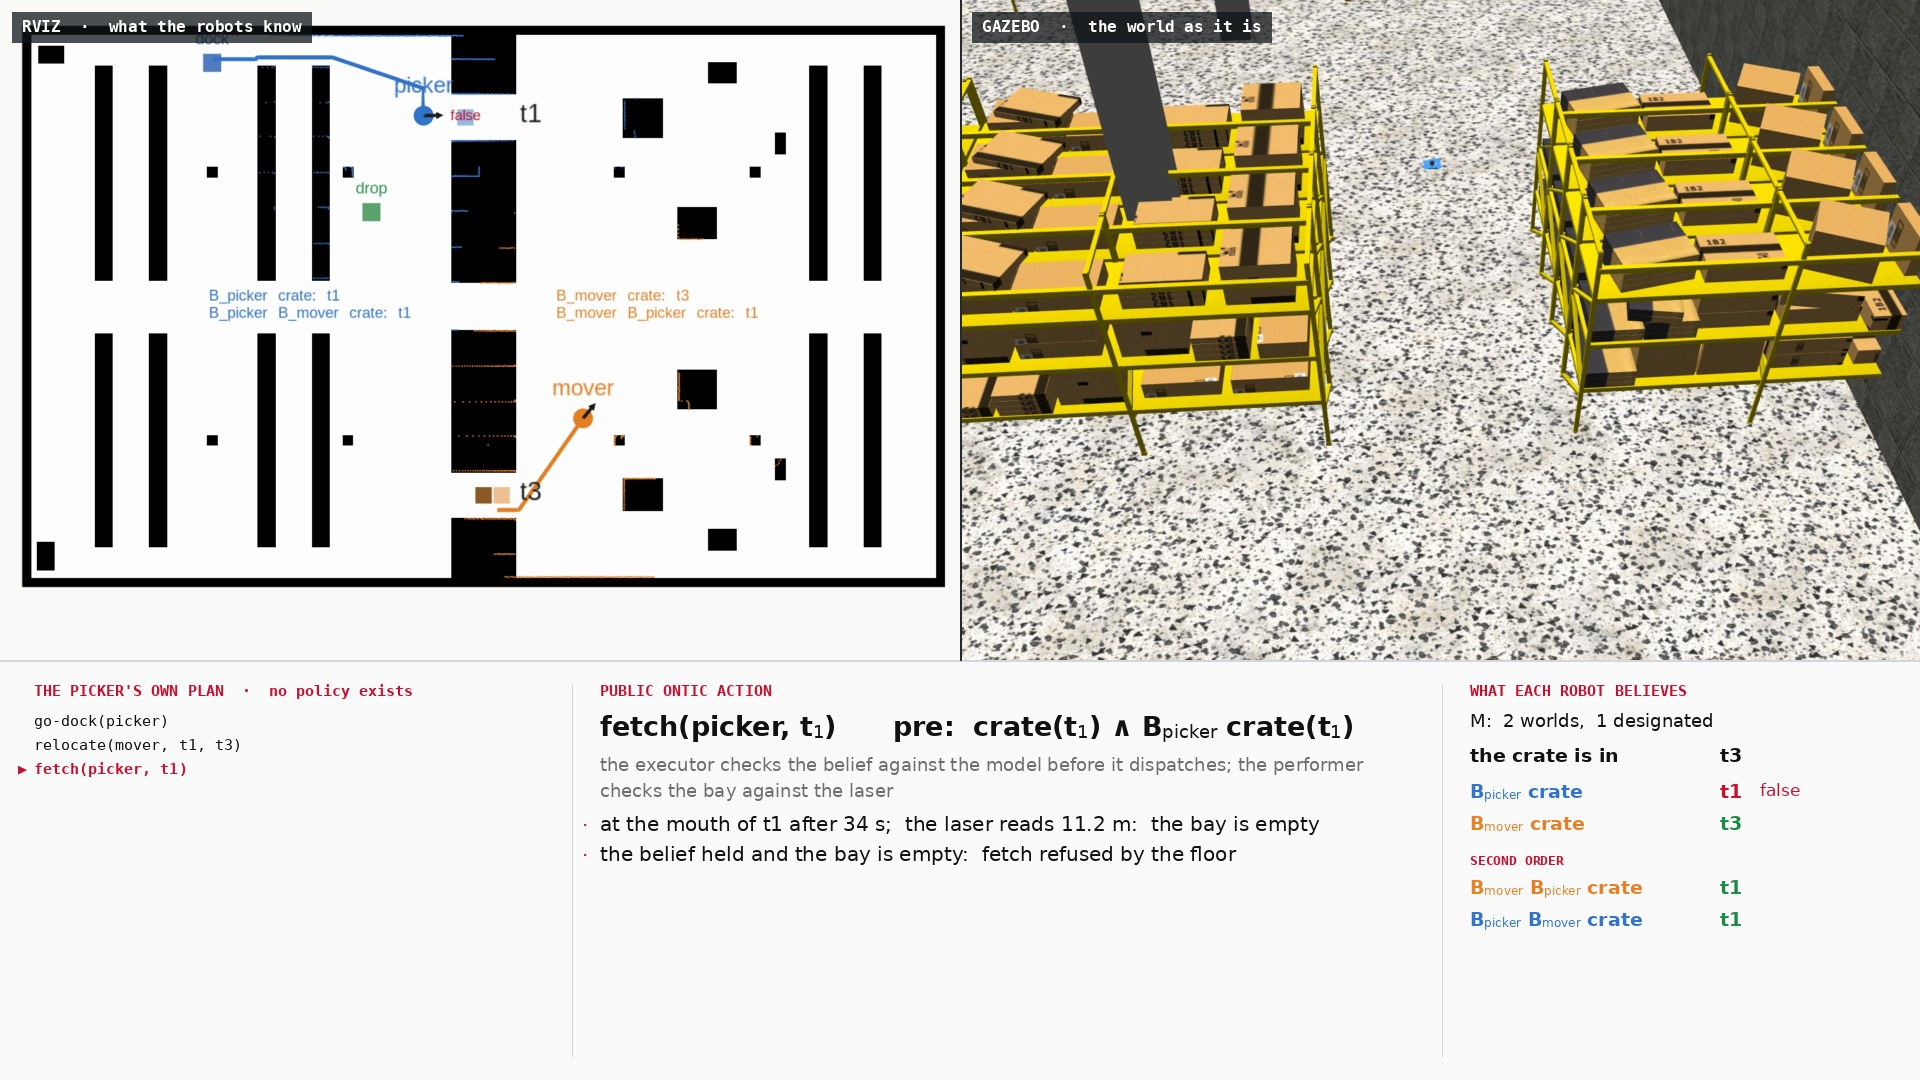
\includegraphics[width=\textwidth]{figures/false_belief_frame_untold.jpg}\\[0.4em]
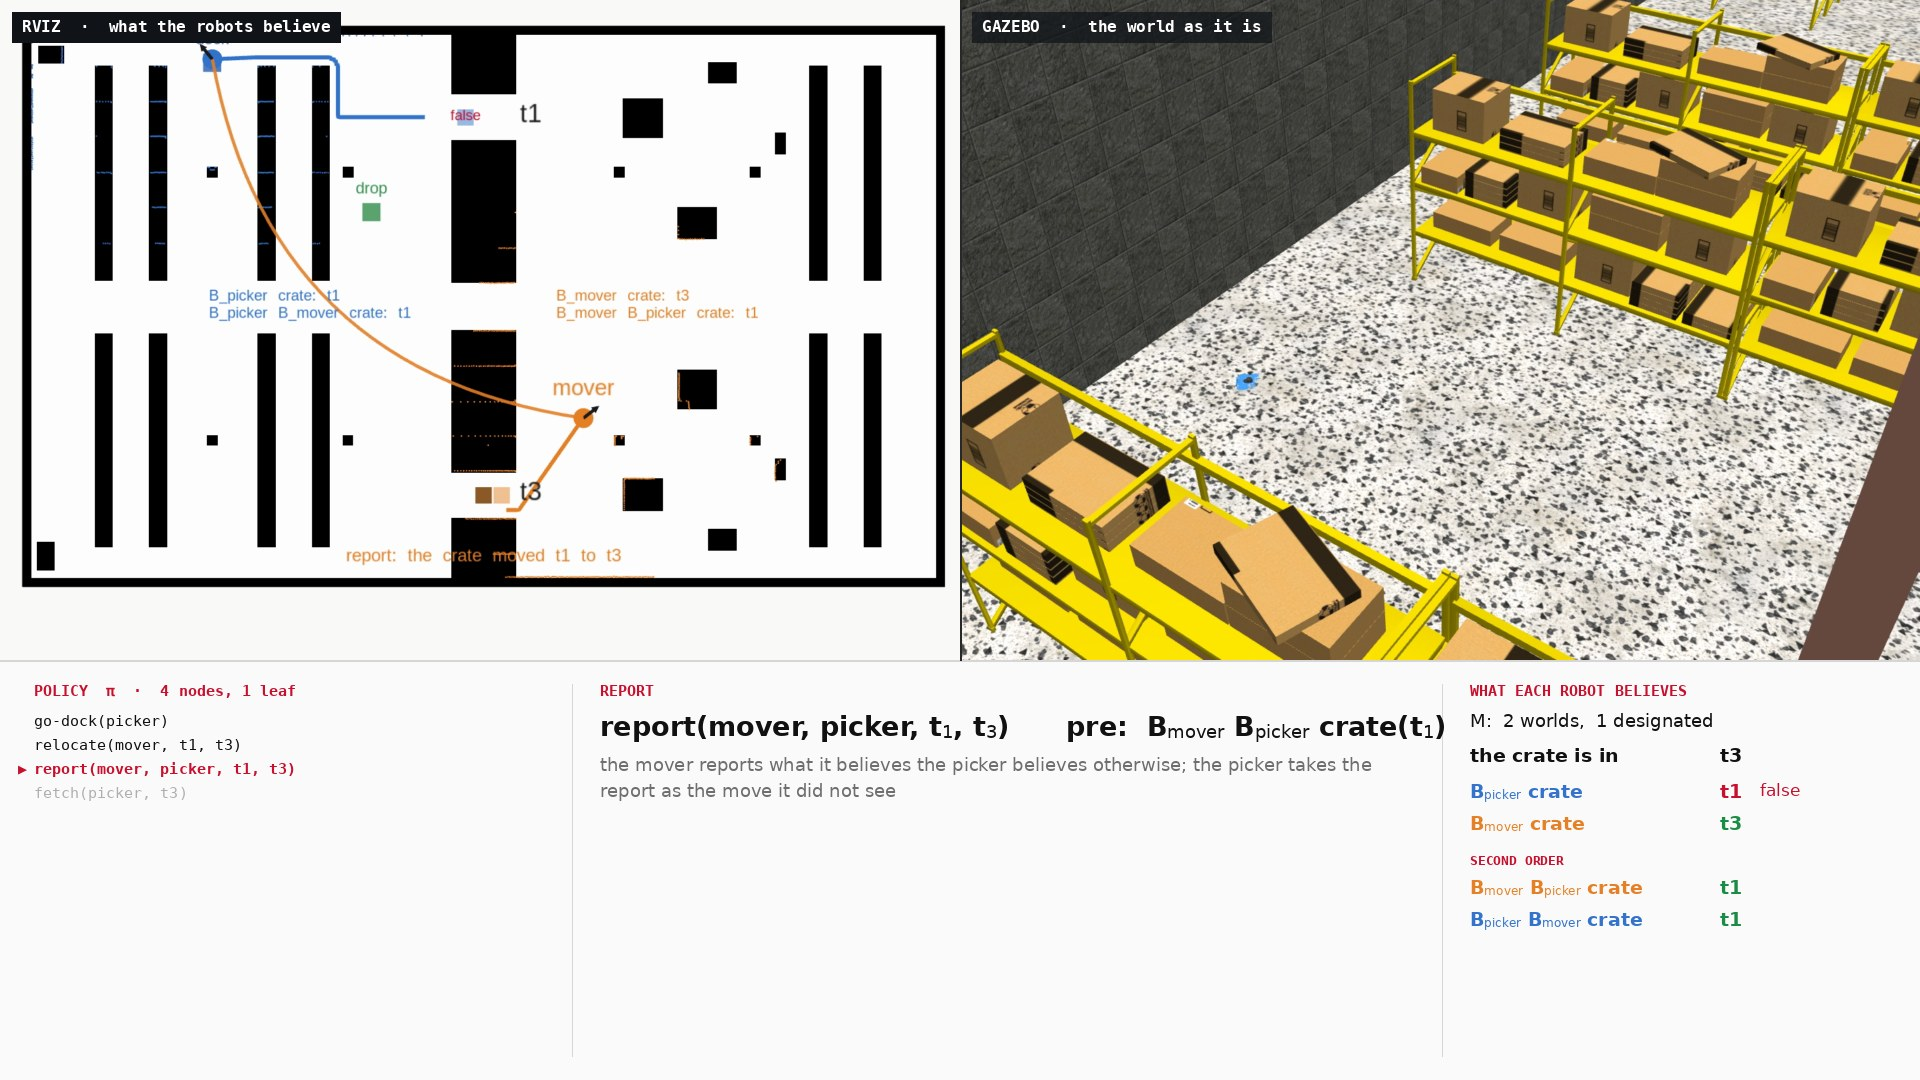
\includegraphics[width=\textwidth]{figures/false_belief_frame_told.jpg}
\caption{Two frames of the film. Above, the untold floor at the refused fetch:
the picker at the mouth of $t_1$, its belief of the crate there marked false,
and the mover's attribution of it in the second-order rows. Below, the told
floor at the report: the arc from the mover to the picker at its dock, a moment
before the picker's belief becomes true.}
\label{fig:frames}
\end{figure}

%  ======================================================================
\section{Defects}
\label{sec:defects}

\paragraph{A policy on every floor} The first solve returned the same policy for
all three instances: look into $t_1$, then fetch from $t_3$. Applied by hand,
the look left the picker with no world, and the precondition
$\Bop{\pk}\crate(t_3)$ of the fetch held vacuously
(Remark~\ref{rem:vacuous}). Aletheia's default keeps such a product, as plank
does. With \code{--consistent-beliefs} the untold instance has no policy, as
Corollary~\ref{cor:untold} says it should not.

\paragraph{A phase the picker could not see pass} With consistent beliefs
required, the told instance then had no policy either. The relocation's event
$\sigma$ was trivial, so the phase atom that $\delta$ clears stayed set in the
world the picker believed, and the fetch, which requires it cleared, had no
world to apply to there: the picker's relation emptied at the fetch. The same
leak had made the doubt instance's look decisive for the wrong reason, since
the look's events also require the phase cleared and so removed the world in
which nothing had moved. $\sigma$ now clears the phase
(Definition~\ref{def:relocation}).

\paragraph{The tracked model keeps a collapse} The epistemic state applies
updates with \code{Ignore}. Had the picker looked into $t_1$ on the untold
floor, the tracked model would have left it believing everything, and every
belief requirement the executor checked afterwards would have held. The
untold run sends the picker to fetch, and the fetch is checked against the
floor, which refuses it. A run that observes as well as acts on a false belief
would need the epistemic state to refuse the update as the planner does.

%  ======================================================================
\section{What the runs establish}
\label{sec:established}

That a false belief, and another agent's attribution of it, can be computed by
the product update an executor maintains during a run, from an event model in
which one robot does not observe a move; and that the attribution predicts
where the robot will go. On the untold floor the mover's model placed the
picker's belief in $t_1$, and the picker drove to $t_1$.

That an observation contradicting a belief has no consistent outcome in this
logic, and that a planner which refuses inconsistent updates finds no policy
where the only way to the goal would pass through one, while a planner which
keeps them finds a policy that works only because a robot believes everything.

And that a report taken as news of the move, and not as an announcement of the
place, repairs the belief consistently and leaves the location common belief;
while a robot that allows a move it does not see is never wrong and needs no
report, only a look.

%  ======================================================================
\section{Directions for the next iteration}
\label{sec:next}

\paragraph{Revision} Plausibility models~\cite{baltag2008} order the worlds an
agent considers by how plausible it finds them, and an observation the most
plausible worlds rule out moves belief to the most plausible worlds it allows.
With them the untold picker, finding $t_1$ empty, would come to believe the
crate somewhere else, and the untold floor would have a policy: look, then
fetch from wherever revision puts the crate.

\paragraph{A mover with a reason} The report is in the policy because the
planner needs it. A mover whose own goal is served by the picker succeeding,
and whose report has a cost, would put the false-belief test in the agent's
decision and not in the planner's search.

\paragraph{The tracked model} The epistemic state could refuse an update that
leaves a robot with no world, as the planner does, and report it as a reason to
replan.

%  ======================================================================
\begin{thebibliography}{9}
\bibitem{baltag2008} A.~Baltag and S.~Smets.
  A qualitative theory of dynamic interactive belief revision.
  In \emph{Logic and the Foundations of Game and Decision Theory (LOFT 7)},
  Texts in Logic and Games 3, pages 11--58. Amsterdam University Press, 2008.
\bibitem{baltag1998} A.~Baltag, L.~S. Moss and S.~Solecki.
  The logic of public announcements, common knowledge, and private suspicions.
  In \emph{Proceedings of TARK VII}, pages 43--56, 1998.
\bibitem{baroncohen1985} S.~Baron-Cohen, A.~M. Leslie and U.~Frith.
  Does the autistic child have a ``theory of mind''?
  \emph{Cognition}, 21(1):37--46, 1985.
\bibitem{bolander2018} T.~Bolander.
  Seeing is believing: formalising false-belief tasks in dynamic epistemic logic.
  In \emph{Jaakko Hintikka on Knowledge and Game-Theoretical Semantics},
  Outstanding Contributions to Logic 12, pages 207--236. Springer, 2018.
\bibitem{bolander2011} T.~Bolander and M.~B. Andersen.
  Epistemic planning for single- and multi-agent systems.
  \emph{Journal of Applied Non-Classical Logics}, 21(1):9--34, 2011.
\bibitem{vanditmarsch2007} H.~van Ditmarsch, W.~van der Hoek and B.~Kooi.
  \emph{Dynamic Epistemic Logic}. Springer, 2007.
\bibitem{wimmer1983} H.~Wimmer and J.~Perner.
  Beliefs about beliefs: representation and constraining function of wrong
  beliefs in young children's understanding of deception.
  \emph{Cognition}, 13(1):103--128, 1983.
\end{thebibliography}

%  ======================================================================
\section*{Reproduction}

\begin{lstlisting}
ros2 launch false_belief_demo false_belief_launch.py floor:=told
ros2 launch false_belief_demo false_belief_launch.py floor:=untold
ros2 launch false_belief_demo false_belief_launch.py floor:=doubt
bash tools/validate.sh                                   # six checks, no simulator
bash tools/record_demo.sh told   /tmp/raw_told.mkv   /tmp/run_told.log
bash tools/record_demo.sh untold /tmp/raw_untold.mkv /tmp/run_untold.log
bash tools/record_demo.sh doubt  /tmp/raw_doubt.mkv  /tmp/run_doubt.log
\end{lstlisting}

\end{document}
